\subsubsection{Selección de tarjeta de desarrollo}

Debido al proceso de compostaje se requiere que la tarjeta de desarrollo sea capaz de leer y procesar la información de los sensores de entrada, así como también ser capaz de  procesar toda esta información para hacer una toma de decisiones, se requiere que la tarjeta  de desarrollo contenga  varios multihilos para realizar todas las operaciones para las que  se debe de encargar.

En el mercado se pueden encontrar diferentes opciones, cada una con características que pueden afectar el desempeño completo de los sistemas, como pueden ser el voltaje de alimentación, los pines de comunicación disponibles, el tamaño  y el precio. 

Para realizar el análisis y la toma de decisiones del sistema, se optó por un sistema de matrices de selección \cite{matselec32}, en el cual se realizo una ponderación numérica para evaluar cada una de las opciones que se consideraron para satisfacer las necesidades del sistema.

Para este caso en particular se tomaron en cuenta criterios como el numero de pines, el costo que tiene, si esta disponible, sus dimensiones así como la posibilidad de conectarse a internet. 

Se realizo la ponderación de las opciones, como se ve a detalle en el apéndice  \ref{Ap:Eje Seleccion}, donde se realiza la matriz de selección de la unidad de procesamiento.  Donde el resultado de la selección fue la tarjeta ESP32.

Esta tarjeta ofrece muchas ventajas en cuanto a la frecuencia de trabajo, para la aplicación de multitareas, también cuenta con su amplia cantidad de pines digitales para interactuar con los elementos de adquisición. Por último, es una tarjeta compatible con el entorno de arduino, lo que hace mas intuitiva su programación. Todas sus características están en la tabla \ref{tab:ESP32 CAR}

\begin{table}[h!]
    \centering
    \caption{Características de la ESP32}
        \begin{tabular}{ |c|c|c|c| } 
            \hline
            \multirow{7}{8em}{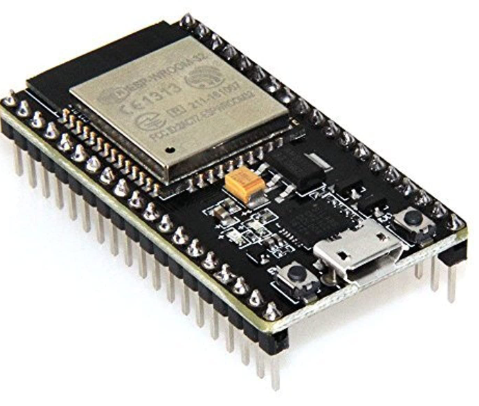
\includegraphics[scale=0.2]{images/Capitulo 4/3.1.1/S1/esp.png}} & \cellcolor[rgb]{ .851,  .851,  .851}Alimentación & \cellcolor[rgb]{ .851,  .851,  .851}3.3 V a 5 V \\ 
            & Microcontrolador & Tensilica Xtensa 32-bit LX6 \\ 
            & \cellcolor[rgb]{ .851,  .851,  .851}Corriente de operacion & \cellcolor[rgb]{ .851,  .851,  .851} 20 a 240 mA \\ 
            & Pines de alimentación & GPIO 24 \\
            & \cellcolor[rgb]{ .851,  .851,  .851}Dimensiones & \cellcolor[rgb]{ .851,  .851,  .851} 51 x 23 mm \\
            & Frecuencia de trabajo & 240 M Hz \\
            & \cellcolor[rgb]{ .851,  .851,  .851}Conexión inalámbrica & \cellcolor[rgb]{ .851,  .851,  .851} Bluetooth y Wi-Fi\\
             \hline
        \end{tabular}
    \label{tab:ESP32 CAR}%
\end{table}